 % if your latex compiler failed to compile, uncomment the command below:
\RequirePackage[2020-02-02]{latexrelease}
\documentclass[sigconf,anonymous]{clv3}
\usepackage{hyperref}
\usepackage[dvipsnames]{xcolor}
\usepackage{natbib}
\definecolor{darkblue}{rgb}{0, 0, 0.5}
\definecolor{red}{rgb}{0.7, 0.005, 0.15}
\hypersetup{colorlinks=true,citecolor=darkblue, linkcolor=darkblue, urlcolor=darkblue}
\usepackage[nameinlink]{cleveref}
%This is where to comment out if you want to remove comments from being visible in the paper:
%\usepackage[textsize=tiny] %comment out
\usepackage[textsize=tiny,disable]
{todonotes}
\newcommand{\note}[4][]{\todo[author=#2,color=#3,size=\scriptsize,fancyline,caption={},#1]{#4}} % 
%\newcommand{\noindentaftertodo}{\iftodonotes{\noindent}{}}
\newcommand{\zee}[2][]{\note[#1]{Z}{olive!40}{#2}}
\newcommand{\Zee}[1]{\zee[inline]{#1}}%\noindentaftertodo}
\newcommand{\lexi}[2][]{\note[#1]{L}{cyan!40}{#2}}
\newcommand{\Lexi}[1]{\lexi[inline]{#1}}%\noindentaftertodo}
\newcommand{\arno}[2][]{\note[#1]{A}{yellow!40}{#2}}
\newcommand{\Arno}[1]{\arno[inline]{#1}}%\noindentaftertodo}
\newcommand{\eddie}[2][]{\note[#1]{E}{red!40}{#2}}
\newcommand{\Eddie}[1]{\eddie[inline]{#1}}%\noindentaftertodo
\newcommand{\nik}[2][]{\note[#1]{N}{purple!40}{#2}}
\newcommand{\Nik}[1]{\nik[inline]{#1}}%\noindentaftertodo}

\definecolor{lightblue}{RGB}{93,162,252}

% test compatibility with algorithmic.sty
%\usepackage{algorithmic}

%\issue{1}{1}{2024}
\runningtitle{Whitepaper on Ethical Research with LLMs}
%\runningauthor{Ungless et al.}

\begin{document}

\title{\textsc{Ethics Whitepaper}: Whitepaper on Ethical Research with Large Language Models}

%\iffalse
\author{Eddie L. Ungless}
\affil{University of Edinburgh}

\author{Nikolas Vitsakis}
\affil{Heriot-Watt University}

\author{Zeerak Talat}
\affil{University of Edinburgh}

\author{James Garforth}
\affil{University of Edinburgh}

\author{Björn Ross}
\affil{University of Edinburgh}

\author{Arno Onken}
\affil{University of Edinburgh}

\author{Atoosa Kasirzadeh}
\affil{University of Edinburgh}

\author{Alexandra Birch\thanks{10 Crichton Street, EH89AB, UK, a.birch@ed.ac.uk}}
\affil{University of Edinburgh}
%\fi



\maketitle

\begin{abstract}
This whitepaper offers an overview of the ethical considerations surrounding research into or with large language models (LLMs). As LLMs become more integrated into widely used applications, their societal impact increases, bringing important ethical questions to the forefront. With a growing body of work examining the ethical development, deployment, and use of LLMs, this whitepaper provides a comprehensive and practical guide to best practices, designed to help those in research and in industry to uphold the highest ethical standards in their work.

\end{abstract}


\section{Introduction}
\noindent\textbf{\textit{Motivation and intended audience of this whitepaper}}
\newline


As large language models (LLMs) grow increasingly powerful, their advancements in natural language understanding and generation are impressive \citep{min_recent_2023}. However, mitigating the risks they present remains a complex challenge, and categorising these risks is a crucial aspect of ethical research related to LLMs~\cite{weidinger2022taxonomy}. Key concerns include the potential to perpetuate and even amplify existing biases present in training data ~\citep{gallegos2024bias}, the challenges in safeguarding user privacy ~\citep{yao2024survey}, hallucination or incorrect responses~\citep{abercrombie-etal-2023-mirages, xu2024hallucination}, malicious use of their powerful capabilities \citep{cuthbertson_chatgpt_2023}, and infringement of copyright~\citep{Lucchi_2023}. Given that many of these ethical challenges remain unresolved, it is essential for those involved in developing LLMs and LLM-based applications to consider potential harms, particularly as these models see broader adoption.

Several frameworks have already been developed to address AI ethics and safety. For example The U.S. National Institute of Standards and Technology (NIST) has a AI Risk Management Framework (RMF)~\footnote{\url{https://www.nist.gov/itl/ai-risk-management-framework}}, which provides broad guidelines for managing AI-related risks. NIST has also recently released a document outlining specific risks and recommended actions for Generative AI~\footnote{\url{https://nvlpubs.nist.gov/nistpubs/ai/NIST.AI.600-1.pdf}}. While widely adopted, the NIST guidelines are voluntary. In contrast, the EU AI Act~\footnote{\url{https://digital-strategy.ec.europa.eu/en/policies/regulatory-framework-ai}} represents a legally binding regulatory framework designed to ensure the safe and ethical use of AI within the European Union. It emphasises transparency, human oversight, and the prevention of discriminatory outcomes, with the goal of protecting fundamental rights and promoting trustworthy AI.  

The NIST AI RMF and EU AI Act are broad, focusing on AI deployment and risk management across industries. There are other frameworks which are more research-focused, guiding ethical considerations in academic AI work. For example the Conference on Neural Information Processing Systems (NeurIPS) Ethics Guidelines~\footnote{\url{https://neurips.cc/public/EthicsGuidelines}} evaluates AI research for ethical concerns as part of the paper submission process.
A similar effort from the Association of Computational Linguistics (ACL) has created an Ethics Checklist\footnote{\url{https://aclrollingreview.org/responsibleNLPresearch/}} which guides authors in addressing ethical implications, including limitations, and correct treatment of human annotators.

Despite there being a number of frameworks for the ethical development of AI, we believe that there is still a need for a practical whitepaper focused on the needs of a practitioner working with LLMs. This whitepaper presents insight and pointers to the most relevant ethical research, as it relates to each of the steps in the project lifecycle. It provides more detail than the guidelines of NeurIPS and ACL, but is more ``digestible'' and directly applicable to research with LLMs than the NIST frameworks or the EU AI act. We hope this whitepaper will prove valuable to all practitioners, whether you are looking for succinct best practice recommendations, a directory of relevant literature, or an introduction to some of the controversies in the field. 





\section{Overview}
\begin{figure}
    \centering
    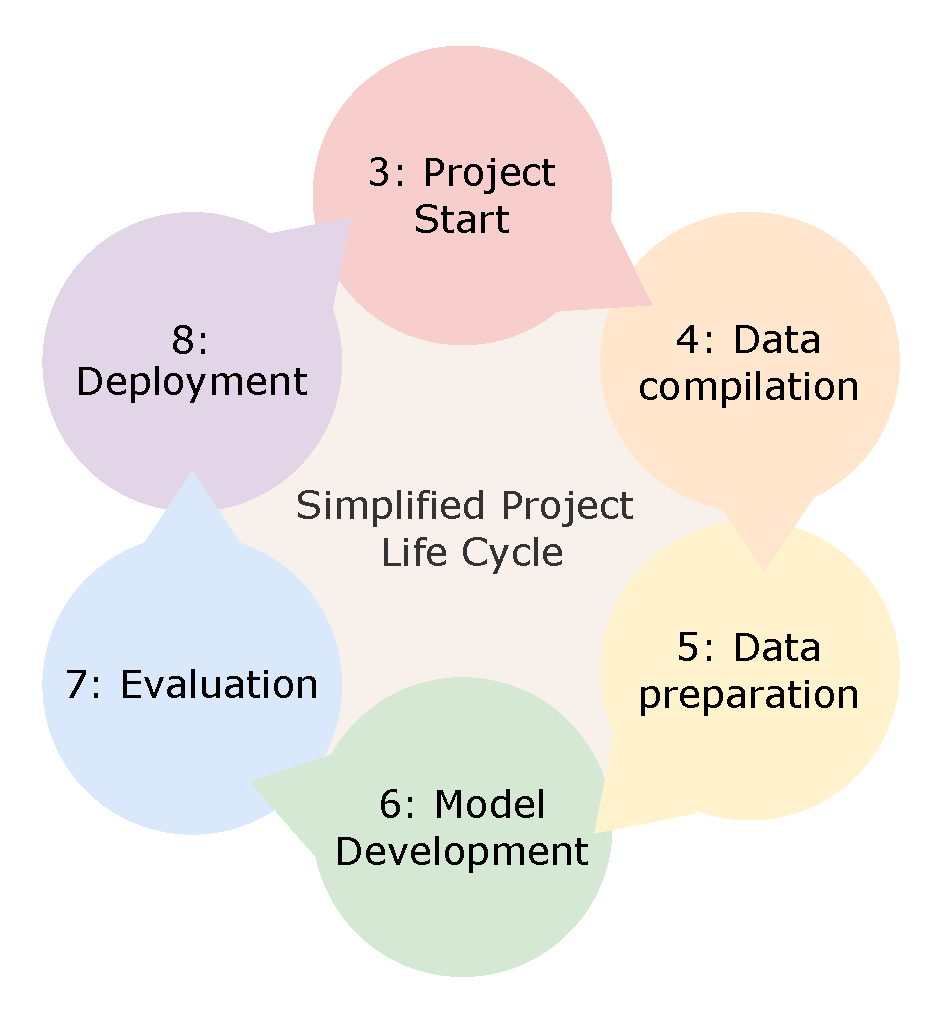
\includegraphics[scale=0.4]{whitepaperstructure.pdf}
    \caption{Diagram showing simplified project lifecycle that forms the structure of this paper.}
    \label{fig:paperstructure}
\end{figure}
%\textcolor{ForestGreen}{Eddie}
This document is structured around a (simplified) project lifecycle, depicted in \Cref{fig:paperstructure}. Our aim for this whitepaper is for it to be used as a reference guide throughout a project, rather than for post-hoc reflection. We begin in \Cref{sec:start} by outlining the importance of ethics and discussing themes relevant to the entire development life cycle.
In \Cref{sec:comp} we consider best practice for data collection and sharing.
Next, in \Cref{sec:prep} we discuss ethical aspects of data preparation, such as cleaning and labelling.
We then turn towards model development in \Cref{sec:modeldev}, focusing on questions of model design, addressing social biases and model alignment.
Following a common develop-then-test structure, we then consider ethical issues related to performance and harm evaluation in \Cref{sec:eval}.
Finally in \Cref{sec:deploy}, we examine the questions of ethics that arise in deployment contexts. You should of course adapt the order you consult these sections to your needs e.g. those finetuning an existing LLM may wish to consult \Cref{sec:modeldev} on Model Development (which has advice for model selection) before Section \hyperref[sec:comp]{4} on Data Compilation (for guidance on compiling finetuning data). However, we recommend every practitioner starts with \Cref{sec:start}, as this has vital guidance for all projects. 

At the end of each Section we give key resources, namely concrete \textcolor{ForestGreen}{do's} and \textcolor{red}{don'ts} for ethical research, relevant to that stage on the project, and tools to guide ethical work. 

%\Lexi{Overview at the moment is very short - perhaps it could fit into Section 1? Also the blue arrow of Finetuning is not very clear to me - I don't feel like it adds much. Also - is there a place that we discuss what the risks are and specifically how to mitigate them? I know others might have done this better but it is not clear where these are. } Lexi: OK happy to move forward on this
%\Eddie{Agree overview can be added to intro but keeping as separate section to section numbers remain same as in email. I have clarified in overview where mitigation lies. Risks discussed in next section. Figure updated}
%\Nik{I prefer the way they are now, it's a place where people can refer back to if they need to find their way around, but am also happy to change merge with intro}

\section{Project Start}\label{sec:start}
\noindent\textbf{\textit{A quick overview of the broad-reaching ethical implications of LLMs}}\newline

\noindent 
The social risk of generative AI, and LLMs can have wide-reaching effects from representational harms to safety concerns, which has been widely recognised \citet[see e.g.,][]{weidinger_ethical_2021,bender_dangers_2021,uzun_are_2023,wei_ai_2022}.
This recognition has given rise to a large number of efforts seeking to evaluate their risks and actualised harms, each effort presenting its own limitations~\cite{Solaiman_Evaluating_2024, goldfarb-tarrant_this_2023, blodgett_language_2020}.
Nevertheless, efforts towards developing technologies that minimise harms, in particular to marginalised communities, are vital.
Best efforts require considering a wide range of topics and questions that must be adapted to each individual application and deployment context. In this Section we explain why ethics is relevant to all practitioners (\Cref{subsec:who}), then highlight resources to aid in the initial discovery process (\Cref{subsec:ideation}). We also lay out best practice that will be valuable to all those working with language technologies, namely related to working with stakeholders, and environmental considerations (\Cref{sec:stakeholders} and \Cref{subsec:energy}).


\subsection{Who needs ethics?}\label{subsec:who}
\noindent\textbf{\textit{Everyone needs ethics}} \\

\noindent As computer science becomes pervasive in modern lives, so too does it become intertwined with the experience of those lives. Decisions made by researchers and developers compound together to influence every aspect of the technical systems which ultimately govern how we all live. This is often at a scale, or level of complexity, which make it impossible to seek clear resolutions when outcomes are harmful \citep{van2020embedding, kasirzadeh2021reasons, miller2021technology, birhane_values_2022, santurkar2023whose, pistilli2024civics}. 

Technical artefacts are inherently political \cite{winner_artifacts_1980}, because they further entrench certain kinds of power e.g. marginalised peoples' data is often used without consent or compensation (see \Cref{sec:whose}); technology typically works best for language varieties associated with whiteness \citep{blodgett_racial_2017}; benchmarks are published which are biased against minorities \citep{buolamwini_gender_2018}. Unfortunately, the training and work cultures of computer scientists often condition us to believe we are beyond politics \citep{malazita2019infrastructures}, because the ``objective'' or abstractive nature of our work seems to absolve us of having to consider issues of our technologies in the world \citep{talat_disembodied_2021} – when dealing with code and numbers it becomes easier to forget about the real humans who are impacted by
our design choices. LLMs are no exception \citep{leidner_ethical_2017}, though their recent rise in prevalence has made their ethical dimensions more salient (and more vital to address). 

Technical work should be considered interdisciplinary by its very nature, as it requires an understanding of the physical and social systems that technical artefacts must interact with in order to achieve their function. Experts exist in all of these other areas of study, as well as their intersections, but very often our lack of appreciation for their expertise, or lack of shared language, impede us from seeking them out. This is especially true for expertise in the social sciences and philosophy \citep{raji2021you, inie_idr_2021, danks2022digital}.  

There is a tendency to assume that social and ethical issues are someone else’s problem \citep{widder2023dislocated}, but this is not the case! If you do not reflect on your design decisions as you make them then you are complicit in the avoidable consequences of those decisions \citep{talat_disembodied_2021}. The decision to follow a code of ethics \cite{mcnamara2018does} or employ a pre-packaged ethical toolkit, does not immediately solve the problem because these decisions require a level of ethical reflection to be effective \citep{wong_seeing_2023}.

\subsection{Laying the Groundwork}\label{subsec:ideation}
\noindent\textbf{\textit{Resources to ensure ethical issues considered from the beginning}}\\

It is important to think about ethics from the very beginning, in order to be able to question all aspects of the project, including if specific tasks should even be undertaken.  One way of doing this is by using ethics sheets \citep{mohammad_ethics_2022}, which are sets of questions to ask and answer before starting an AI project. It includes questions like ``Why should we automate this task?'', and ``How can the automated system be abused?''. 
An alternative is using the Assessment List for Trustworthy Artificial Intelligence (ALTAI)\footnote{\url{https://ec.europa.eu/newsroom/dae/document.cfm?doc_id=68342}}, which is a tool that helps business and organisations to self-assess the trustworthiness of their AI systems under development. The European Commission appointed a group of experts to provide advice on its artificial intelligence strategy and they translated these requirements into a detailed Assessment List, taking into account feedback from a six month long piloting process within the European AI community. 
You could use question sets such as these to ensure ethical considerations are present from the start of your project. 

Regulated industries such as aerospace, medicine and finance have critical safety issues to address, and a primary way these have been addressed is using auditable processes throughout a project. Audits are tools for interrogating complex processes, to determine whether they comply with company policy and industry standards or regulations~\citep{liu2012enterprise}. \citet{raji_closing_2020} introduce a framework for algorithmic auditing that supports artificial intelligence system development, which is intended to contribute to closing the gap between principles and practice. They map out the process of implementing an internal audit for use during the development process (as opposed to post-hoc audits), which you can adopt to ensure responsibility for upholding ethical values is clearly assigned. A formal process such as this can help by raising awareness, assigning responsibility, and improving consistency in both procedures and outcomes \citep{leidner_ethical_2017}. At the very least, your organisation should establish an ethics review board to evaluate new products, services, or research plans~\citep{raji_closing_2020}.

Foreseeing the downstream effects of deploying an AI system is challenging and requires grappling with complex contexts that even seemingly simple AI technologies may interact with. The ideation tools discussed above will help in anticipating possible effects. You will also benefit from reading about likely risks, for example in \citet{Solaiman_Evaluating_2024} (see also \Cref{subsec:harms}). Further resources include \citet{bucinca_aha_2023} who propose AHA! (Anticipating Harms of AI) which combines crowd-workers and LLMs to surface a wide variety of potential harms.

\citet{weisz_toward_2023} outline design principles for developing generative AI applications, grounded in the concept of generative variability, which highlight that generative AI systems produce outputs which can vary in quality and character. The design principles emphasize designing for multiple, imperfect outputs. Their final design principle is proactively mitigating potential harms such as producing inappropriate content or displacing human workers. You can use these design principles to help you make thoughtful decisions when developing innovative LLM applications.

Finally, exploring ethics in a global context has the added challenge of balancing between the valuing of cultural diversity and the respect for human rights. \citet{reid_ethics_2021} develop a framework for collaboration that respects the variety of people and cultures that might be involved in research and encourages researchers to consider their perspectives from ideation right through to the legacy left by the project. 

\subsection{Stakeholders}\label{sec:stakeholders}
\noindent\textbf{\textit{Best practice for thinking about and working with stakeholders}}\\

\noindent Given the vast amounts of training data required and the wide-reaching applications of LLMs, every project will have many stakeholders e.g. those who provide the data \citep{havens_situated_2020}, end-users of the application \citep{yang2023impact}, or those a model will be used \emph{on}, who are often given limited power to influence design decisions e.g. migrants \citep{nalbandian_eye_2022}. A vital early step is identifying key direct stakeholders and establishing the best ways to work with them in order to build systems that are widely beneficial, and this will be highly context dependent \citep{sloane_participation_2022}. The ideation toolkits detailed above will help you to identify stakeholders, and can be used alongside existing taxonomies e.g. \citep[i.a.]{lewis_global_2020,langer_what_2021, bird_typology_2023, havens_situated_2020}. 
Crucially, stakeholders should be identified before development, so they can (if they wish) be involved in co-production, or object to proposed technologies \citep{munn_uselessness_2022}. \citet{kawakami_situate_2024} present a toolkit for early stage deliberation with stakeholders with question prompts, while \citet{caselli_guiding_2021} provide 9 guiding principles for effective participatory design (which involves mutual learning between designer and participant) in the context of NLP research. 
Input from stakeholders is vital for constructing Value Scenarios, a methodology which predicts the likely impact of a proposed technology \citep{nathan_value_2007}, as in \citet{haroutunian_ethical_2022}'s paper on low-resourced machine translation. 
\citet{havens_situated_2020} invite us to work collaboratively with stakeholders to understand who or what is included in our research, and who is excluded, while \citet{jurgens_just_2019} explain how working with affected communities enables the establishment of research norms that are context-informed and sensitive to the needs of the community (e.g., establishment and use of appropriate language \citep{jurgens_just_2019}).

You must consider power relations between stakeholders \citep{havens_situated_2020}, including between yourself and the stakeholders. Those of marginalised genders or ethnicities may not be represented in your research team \citep{west_discriminating_2019}, which can influence researcher-stakeholder relations (e.g. lack of cultural knowledge, greater power imbalance \citep{madaio2022assessing,fukuda-parr_emerging_2021,haque2024we}). Reflexive considerations about a researcher's own power are rare in computer science research \citep{ovalle_factoring_2023, devinney_theories_2022} but can help establish the limitations of your work \citep{liang_embracing_2021,liang_reflexivity_2021}. This is particularly important when reaching out to marginalised communities, as these relationships can be even unintentionally exploitative. For example marginalised communities are often not fairly compensated for their participation \cite{sloane_participation_2022}, or are only invited to partake in feedback but not co-production \cite{sloane_participation_2022, ungless_stereotypes_2023}.

When working on technologies for indigenous and endangered languages, sensitive stakeholder collaboration is particularly important \citep{bird_decolonising_2020, liu_not_2022, mahelona_openais_2023}. Work on stakeholder engagement in NLP can learn much from the Indigenous Data Sovereignty movement \citep{sloane_participation_2022}, which we return to in \Cref{sec:whose}. 

\subsection{Energy Consumption}\label{subsec:energy}
\noindent\textbf{\textit{Consider the ethics of the environment}}\\

\noindent Throughout the life cycle of a project, you should consider the energy consumption of your model, which relates to data sourcing practices, model design, choice of hardware, and use at production. \citet{strubell_energy_2019} suggest that model development likely contributes a ``substantial proportion of the... emissions attributed to many NLP researchers''. 
\citet{strubell_energy_2019} call for more research on computationally efficient hardware and algorithms, and the standardised calculation and reporting of finetuning cost-benefit assessments, so researchers can select efficient models to finetune (models that are responsive to finetuning).
Similar recommendations are made by \citet{henderson_towards_2020}, who also provide a framework for tracking energy, compute and carbon impacts. 
\citet{patterson_carbon_2022} provide best practice for reducing the carbon footprint, including the development of sparse over dense model architectures and the use of cloud computing that relies on renewable energy sources. 
\citet{bannour_evaluating_2021} provide a taxonomy of tools available to measure the impact of NLP technologies. 

Sasha Luccioni and colleagues have in particular championed the accurate reporting of the carbon emissions of ML systems including LLMs \citep{luccioni_estimating_2023, luccioni_counting_2023, wang_energy_2023, luccioni_power_2024, dodge_measuring_2022, lacoste_quantifying_2019}. 
They find ``better performance is not generally achieved by using more energy'' across a range of NLP tasks \citep{luccioni_counting_2023}. 
They provide a Python package for tracking the carbon impact of a given codebase \citep{courty_mlco2codecarbon_2024}, and a procedure to measure the energy consumption of LLMs during finetuning \cite{wang_energy_2023}. 
\citet{wang_energy_2023} note one way to reduce energy consumption at fine-tuning and inference is to use compression techniques, such as pruning and distillation, the additional cost of distilling quickly offset by these models being more energy efficient. However you should note that compression techniques can impact fairness as we discuss further in Section \cref{subsec:design}; clearly, compromises must be made. \citet{luccioni_power_2024} also highlight that huge multi-purpose models have far greater cost at inference, so if classification is required it would be more energy efficient to use a task-specific model than rely on prompting. 

\Zee{Takeaways for conclusion:\\
The energy consumption for training NLP technologies, in particular LLMs, create large carbon outputs, relative to one's daily life otherwise, and it is therefore important to bear in mind.
Several techniques and toolsets exist to help identify the approximate carbon emissions produced when developing models, which researchers can benefit from using. 
Further, more energy efficient models, i.e., smaller models, can have higher performance over less energy efficient models for many NLP tasks~\cite{luccioni_counting_2023}.
This can lead one to favour compressed models, e.g., distilled versions of larger models, however compression techniques can result in exaggerated levels of bias, in comparison to their uncompressed versions.
Beyond the training procedure, it is also worth considering the inference-time costs, as these can significantly contribute to the total carbon emissions produced in the entire lifetime of a system.}

\subsection{Key Resources}
Do's and Don'ts
\begin{itemize}
    \item \textcolor{ForestGreen}{\textbf{Do}} engage with affected communities from the beginning - \textcolor{red}{\textbf{don't}} just ask for their feedback
    \item \textcolor{ForestGreen}{\textbf{Do}} allow for flexibility in project direction as informed by stakeholder input - \textcolor{red}{\textbf{don't}} assume what communities want and need
    \item \textcolor{ForestGreen}{\textbf{Do}} consider the power relations between stakeholders -- \textcolor{red}{\textbf{don't}} forget about the relationships with yourself
    \item \textcolor{ForestGreen}{\textbf{Do}} engage with ethics review boards to ensure oversight, or set one up if necessary - \textcolor{red}{\textbf{don't}} assume because its computer science that moral and political values are out of scope
    \item \textcolor{ForestGreen}{\textbf{Do}} create an internal audit procedure to ensure ethical processes are developed and followed - \textcolor{red}{\textbf{don't}} just leave it to a post-hoc review 
    \item \textcolor{ForestGreen}{\textbf{Do}} consider use of compressed models and cloud resources to minimise energy impact - \textcolor{red}{\textbf{don't}} assume you need energy intensive models for the best performance
\end{itemize}

\noindent Useful Tool(kit)s: 
\begin{itemize}
    \item Ethics sheets to discover harms and mitigation strategies -- \citet{mohammad_ethics_2022}
    \item The Assessment List for Trustworthy Artificial Intelligence (ALTAI) \footnote{\url{https://ec.europa.eu/newsroom/dae/document.cfm?doc_id=68342}}
    \item Internal audit framework to ensure that ethical processes are implemented and followed -- \citet{raji_closing_2020}
    \item Value Scenarios framework to identify likely impact of technology -- \citet{nathan_value_2007}
    \item Guiding principles for effective participatory design -- \citet{caselli_guiding_2021}
    \item Best practice for reducing carbon footprint during training -- \citet{patterson_carbon_2022}
    \item Taxonomy of tools available to measure environmental impact of NLP technologies -- \citet{bannour_evaluating_2021}
    \item Software package to estimate carbon dioxide required to execute Python codebase -- \url{https://github.com/mlco2/codecarbon} 
\end{itemize}
\section{Data compilation}\label{sec:comp}

\noindent\textbf{\textit{Overview of ethically significant impacts of data compilation decisions}} 
\newline


\subsection{Compiling own ``raw'' data}
\noindent\textbf{\textit{Issues with typical practices in data compilation and guidance on best practice.}} 
\newline \\
%\textit{Issues with typical practices in data compilation and guidance on best practice.} 
When collecting data, we have to make deliberate choices about what data to include, or not; the ethical ramifications of these choices should be carefully considered. 
Design biases in data set\eddie{data set or data set} compilation often stem from the creator's positionality \citep{talat_disembodied_2021,santy_nlpositionality_2023}: people with different lived experiences will make different choices. 
Therefore, a useful first step may be to consider your own positionality, what choices you are making and \textit{why}, and to document this - a task that is much easier said than done! However, here we can borrow methods from qualitative fields, such as the social sciences.
In particular, the concept of \textit{reflexivity} can help researchers identify how your own positionality and subjectivity provides a particular view into your work \cite{Jamieson_Reflexivity_2023}.\footnote{For an example of a reflexive practive in the context of NLP research, see \citet{Talat_It_2021}.}

Reflexive research practices can also help to critically examine how we see the data we work with. There is the pervasive notion of data as a natural resource, ready to be exploited.
As \citet{benjamin_what_2021} notes, this metaphor is harmful. 
Data is created by people, and to exploit the data can mean exploiting the people who created it. 
As \citet{rawdata2013} point out: ``raw data is an oxymoron.'' 
For example, the texts we use to train LLMs have been created by someone for a particular purpose, and we reuse them for another. 
The supposedly ``raw'' data has actually already undergone various transformations: from someone's thought to written text, in a particular context and time, and then further to ``data'' that is stripped of its context.
%first from intent to actualisation, by a particular person with a particular subjectivity and location; and second from its initial purpose to being made intelligible for the purposes of the researcher or developer of a given technology that exists to serve another purpose beyond the original intention.
%There really is no such thing as ``raw'' data \citep{rawdata2013}: the texts we train LLMs on have been created by someone else, and we are re-using them for a different purpose.

A common source of ``raw'' data for LLM training is texts that are publicly available on the internet \citep[see e.g.][]{openai2024}. 
The ethics of compiling data for training LLMs is therefore closely linked to the ethics of web crawling which have long been discussed in the context of web search \citep{gold2017robots}. 
%Literature on ``polite'' web crawling goes back to the 1990s and the Web's ``robots exclusion protocol'', which allows website owners to control whether they allow web crawlers dates back to 1994. 
There are clear differences, however, between web search and LLM training, and the social norms established for search should be revisited: we may well conclude that there is data that is ethical to index for search purposes but unethical to copy for LLM training purposes.
As for the ``dark web'' that is not indexed by search engines, ethical issues abound when it comes to scraping this data for the purpose of training LLMs. 
For example, online discussions on social media platforms such as review sites may be appropriate to index, using data from discussion boards where people explicitly seek to hide their identity and avoid association to their person may not be ethical, or even wanted as the data may contain artefacts that are undesirable to encode in LLMs.

Data scraped from the internet is likely to contain sensitive personal information \cite{mieskes_quantitative_2017} (we return to this in \Cref{subsec:clean}) and over-represent certain populations, languages, and speakers \cite{Dunn_Mapping_2020}. This can lead to issues of unfairness; while unfairness can enter a model at many different stages \citep{suresh_framework_2021}, training data selection is certainly one of them. 
For an overview of the types of bias this can result in, see \citet{navigli2023biases}. For another, broader perspective on issues in data set creation, see \citet{paullada_data_2020}.

Of course there are many other potential approaches to obtain data, such as licensing it from rights holders. 
The prospect of holding data from multiple rights holders about millions of data subjects who may be unaware of the data processing, while operating across a variety of jurisdictions, bring up complex questions of big data governance that \citet{jernite_data_2022} have attempted to address. 
The sheer size and diversity of these data sets makes it practically impossible to fully understand them, and filter out unwanted data; \citet{luccioni_whats_2021} propose a number of research directions to address this issue. These rights holders are unlikely to spontaneously undermine their own business models, however, and so those of us licensing from them should be sure to be holding them to high standards.

%\textcolor{ForestGreen}{Bjorn}
%\zee{Also useful to take a look at Raw Data is an Oxymoron by Lisa Gitelman, specifically Chapter one with Virginia Jackson}
%ethics and big data charter \cite{couillault_evaluating_2014}

%\citep{birhane_large_2021}

%End section with link to discusson in \cref{sec:replacehumans} on using LLM to ``replace'' human subjects by creating synthetic data - issues of training on data generated by LLMs \cite{briesch_large_2024, shumailov_AI_2024}

%Could be the place to talk about using crowdsourcing to generate bias data sets but this can be a massive quality issue as critiqued in \citet{blodgett_stereotyping_2021} (and \citet{crawford_excavating_2021} for text-image data set ImageNet)

\subsection{Consent and Safety}\label{sec:whose}
\noindent\textbf{\textit{Issues related to consent, safety and power when compiling data from people.}}
\newline 


\noindent We follow \citet{havens_situated_2020} and \citet{bird_typology_2023} in distinguishing those who produce data from those who are represented in the data (data subjects) (e.g. a tweet might be about another person). Many jurisdictions afford legal protections to both: data producers are protected by copyright laws, which we discuss in \Cref{subsec:share}, while data subjects (can) benefit from privacy legislation. However, different jurisdictions adopt different approaches, some offering far less protection. You should reflect on whether you are doing enough to protect both data producers and subjects, and consider extending protections beyond the extent required by law. Taking due ethical care, beyond what the law requires, is often the best way to build public affection and enthusiasm for new technologies, rather than alienating the communities we design for.

A major issue is lack of consent from data providers and subjects. People are often unaware their public data is being collected for LLMs \citep{kim_propile_2023} (as \citet{scheuerman_human_2023, meng_owning_2021} discuss for other AI technology), or are given insufficient information to consent \citep{winograd_loose-lipped_2022, xiao_bad_2020}. Some large publicly available vision and language data sets have introduced processes for data producers and subjects to have data removed \citep{heikkila_artists_2022}, for example in line with GDPR e.g. LAION.\footnote{\url{https://laion.ai/faq/}} This protection cannot help if the data has already been used to train a model, which may go on to reproduce training data, including Personally Identifiable Information (PII) \citep{lukas_analyzing_2023} and copyright material \citep{karamolegkou_copyright_2023}. You must respect the privacy rights of data producers and subjects (which can be conflicting \citep{kekulluoglu_preserving_2018}), rather than relying on the public to request their data be removed. You should use best practice such as transparent data collection, right to removal and respect of copyright to keep your data as clean as possible.

Best practice for social media data collection involves only storing post IDs, such that deleted posts will not be included in future uses. Even where social media platform policies mention content may be used for research, it is debatable whether this constitutes informed consent \citep{fiesler_remember_2024}. \citet{fiesler_remember_2024} recommend reaching out to community moderators on Reddit to understand privacy expectations, which is also relevant to forums and Facebook groups. \citet{mancosu_what_2020}

%The onus is on you to keep your data clean.\eddie{Are readers going to be turned off by this because it seems impossible given current norms?} \lexi{This does not seem like practical advice - or at all feasible - so yes this might put reader off - how do they keep their data clean? We could say as clean as possible instead}

Data from vulnerable populations or about sensitive topics must be especially carefully handled. \citet{klassen_this_2022} emphasise the importance of cultural competence when using social media data from marginalised groups, to mitigate inadvertent harm. Data de-anonymsation can risk data subject safety \citep{rocher_estimating_2019}. The UK's Information Commissioner's Office provides guidelines based on GDPR which may be useful, for example by identifying the kinds of sensitive data that may need additional security and defining informed consent.\footnote{\url{https://ico.org.uk/for-organisations/advice-for-small-organisations/frequently-asked-questions/data-storage-sharing-and-security/\#whatsecurity}} When gathering data, reflect on what data you need to accomplish the task, and what sensitive data should be excluded. 
\citet{benton_ethical_2017} provide guidelines for compiling social media data for studying health; their guidelines may be useful to those working with social media data across different sensitive tasks, for example, they advise to ``separate annotations from user data''.

Certain communities may be under-represented in your data, due to (a) lack of public online presence (b) small community size (c) problematic data compilation practices \citep{guyan_constructing_2021}. This leads to biased model output (see \cref{sec:debias} and \cref{sec:harmeval}). \citet{markl_mind_2022} provides case studies for evaluating speech data sets for what and who is missing, which can be easily extended to other modalities. When addressing under-representation, care must be taken not to cause harm. It may not be safe for certain communities to be compiled into labeled data sets e.g. queer populations \citep{ungless_stereotypes_2023, sigurgeirsson_just_2024}. Data compilation practices can be exploitative, for example when data producers are not given the knowledge required for informed consent, or when monetary incentives act as a form of coersion \citep{fussell_how_2019, reid_ethics_2021, mahelona_openais_2023}. When compiling data from marginalised populations, the Indigenous data sovereignty movement provides best practice \citep{walter_indigenous_2021}. For example, giving marginalised populations agency in what data is collected about them, and taking into account the worldviews of the affected population. %\citep{walter_indigenous_2021}.%Indigenous data practices discourage extractive capitalist practices - whereby a natural resource (native speaker capabilities) are extracted -- exploited -- for financial gain \cite{mahelona_openais_2023}. 

%Certain communities underrepresented i.e. compiling queer data \citep{guyan_constructing_2021,kevin_guyan_queer_2022,ungless_stereotypes_2023}
%Who is missing? \citep{markl_mind_2022}
%Issues of data security \citep{ungless_stereotypes_2023}
%Exploitation of people for data \citep{fussell_how_2019}
%Indigenous data sovereignty, data as colonisation \citep{walter_indigenous_2021,mahelona_openais_2023, schwartz_primum_2022, bird_decolonising_2020}

\subsection{Sharing and Using data}\label{subsec:share}\noindent\textbf{\textit{Ethical considerations when sharing data or using shared data, including documentation.}}
\newline 

\noindent Training LLMs relies heavily on very large data sets composed of web-crawled data and other data sources.  
A useful position paper~\cite{rogers_just_2021} proposes a checklist for responsible data use and reuse. 
The legal and ethical principles of data collection are complicated by the sheer number of sources of data and jurisidictions. Researchers need to follow legal restrictions, for example by respecting copyright, but this can vary depending on the country.
In addition to copyright, data is frequently protected by ``Terms of Service'' for example by social media companies like X (formerly Twitter). These vary by site and can change over time. Ethical principles such as respecting privacy, allowing reproducibility and doing no harm can also be complicated to follow and even conflicting. How do we respect Twitter users' privacy by not saving their tweets, while allowing other researchers access to our data? The checklist proposed by \citet{rogers_just_2021} advances the discussion towards establishing a single standard for responsible data compilation.

Though we rely heavily on large data sets for training LLMs, there is a significant gap in our understanding of their content, including general statistics, quality, social factors, and the presence of evaluation data i.e. contamination. \citet{elazar_whats_2024} introduces "What's In My Big Data?" (WIMBD), a platform designed to uncover and compare the contents of large text corpora, finding issues of low-quality content, sensitive data and benchmark contamination in ten corpora used in training popular language models, such as C4 and The Pile.
 
One of the biggest contributions researchers can make to the field is publishing new data sets. However, it is very important that future users of these data sets understand why and how they were created in order to use them correctly. Following work detailing how to describe data sets specifically for natural language processing~\cite{bender_data_2018}, a more broadly applicable approach was proposed called datasheets~\citep{gebru_datasheets_2020}. Datasheets are structured documents that provide information about a data set to ensure its appropriate and ethical use, including details on its composition, intended uses, and limitations. This transparency helps users understand the data's context and potential harms.

%ethical implications of data sharing \cite{drugan_shared_2010} - Lexi: interesting but maybe a bit niche - focussing on collaborative data creation efforts
% Ethical implications of shared taks(?) \cite{parra_escartin_ethical_2017} - Lexi: this is more about shared tasks than data use and sharing? 


\subsection{Key Resources}
Do's and Don'ts
\begin{itemize}
    \item \textcolor{ForestGreen}{\textbf{Do}} reflect on and document the decisions you make when collecting data - \textcolor{red}{\textbf{don't}} forget that \textit{how} you collect data transforms it 
    \item \textcolor{ForestGreen}{\textbf{Do}} consider if it is ethical to scrape web content, even for content that is publicly available (e.g., by relying on frameworks of ethical data scraping such as \citet{mancosu_what_2020}) - \textcolor{red}{\textbf{don't}} crawl content that website creators have indicated should not be crawled (e.g. via \texttt{robots.txt} files)
    \item \textcolor{ForestGreen}{\textbf{Do}} consider the subjects of the data - \textcolor{red}{\textbf{don't}} just think about the rights of data producers
    \item \textcolor{ForestGreen}{\textbf{Do}} respect copyright and privacy from the beginning - \textcolor{red}{\textbf{don't}} expect the public to do the work of requesting removal (but give them the option!)
    \item \textcolor{ForestGreen}{\textbf{Do}} provide a datasheet for any data set you produce - \textcolor{red}{\textbf{don't}} forget to document intended use and limitations
    %\item \textcolor{ForestGreen}{\textbf{Do}} compile data from marginalised populations respectfully - \textcolor{red}{\textbf{don't}} assume everyone wants to be in compiled data
\end{itemize}

\noindent Useful Tool(kit)s: 
\begin{itemize}
    %\item Overview of issues in ML data set creation -- \citet{paullada_data_2020}
    %\item Guidelines for compiling sensitive social media data -- \citet{benton_ethical_2017}
    \item Case study structure to identify who is missing from collected data -- \citet{markl_mind_2022}
    \item Best practice from Indigenous data sovereignty movement -- \citet{walter_indigenous_2021}
    \item Checklist for responsible data collection and reuse - \citet{rogers_just_2021} 
    \item API to explore content of popular massive data sets - \citet{elazar_whats_2024} 
    \item Guidelines to create datasheets - \citet{gebru_datasheets_2020}
\end{itemize}
\section{Data preparation}\label{sec:prep}

\noindent\textbf{\textit{Overview of ethically significant impacts of data preparation decisions}}
\newline 


\subsection{``Cleaning'' data}\label{subsec:clean}\noindent\textbf{\textit{Potential ethical issues and best practice for data cleaning e.g. filtering.}}
\newline 

\noindent It is vital that you conduct some ``cleaning'' of training data to minimise the amount of irrelevant (e.g. content from another language, when creating a monolingual model), offensive (e.g. hatespeech, misogyny, violence) or private (e.g. personally identifiable information, PII) content, which would limit model performance or result in harmful output. However, automatically filtering out ``irrelevant'' language data has been shown to introduce racial biases due to the association between ``non-standard'' languages and marginalised ethnic communities (for example African American Aligned English \citep{blodgett_racial_2017}). \citet{jurgens_incorporating_2017} has proposed a methodology for language identification that allows for greater diversity. 

Use of n-gram lists or machine learning based systems to detect and filter out harmful content can both introduce issues of bias \citep{anwar2024foundational}. Word lists may exclude reclaimed slurs and queer identity terms \cite{bender_dangers_2021}. Hate detection models such as Perspective API have been shown to exhibit bias against content by and about marginalised communities \citep{rottger_hatecheck_2021}, and have poor robustness \cite{calabrese_aaa_2021}. Further, filtering out explicitely offensive language may fail to identify subtle forms of implicit harm \cite{gadiraju_i_2023,talat_understanding_2017}, including ``dog whistles''\footnote{\url{https://swu-union.org.uk/2023/01/part-4-dog-whistles-in-context-transphobia/}} that seem innocuous. What data is considered ``dirty'', needing to be cleaned out, is highly subjective \citep{thylstrup_detecting_2020}. It will benefit you to think of data harm as a spectrum rather than a binary category. As such it would be reasonable to ``draw the line'' at different ``levels'' of harm, so whatever decision you make should be justified. Further different kinds of harmful content will benefit from different cleaning techniques. 

\citet{hong_whos_2024} highlight how filtering practices can introduce and reinforce biases (in the context of text-image models) -- which has also been demonstrated for language models \citep{welbl_challenges_2021} -- and provide recommendations for those conducting data filtering more broadly, including justifying your filtering design choices and evaluating chosen filters for bias. \citet{anwar2024foundational} propose relying on data balancing and rewriting in place of data filtering to minimise the unfair impact.

As \citet{subramani_detecting_2023} note, the topic of removing PII from training data for LLMs is ``relatively under-explored'', which is particularly problematic given the tendency of LLMs to memorise and later reveal PII such as email addresses \citep{carlini_extracting_2021}. \citet{subramani_detecting_2023} define risk levels and categories of PI, and provide guidance on how to detect and remove ``character based'' PI (i.e. sequences of numbers or letters that uniquely identify a person such as a credit card number or email address). They find C4 and Pile, widely used crawled training data sets, containing tens of millions of instances of PI. They recommend use of out of the box PI detection tools such as Presidio to find and replace PI with anonymising tokens. 

\subsection{Choice of target labels}\noindent\textbf{\textit{Guidelines for defining target (prediction) label options for your data.}}
\newline 

\noindent Labelling can be thought of as the process of simplifying reality (as approximated in your data) into a format that is readable to an ML system. 
This can introduce a great number of ethical issues. 
The proxy may be an \emph{over}-simplification~\cite{Mulvin_Proxies_2021}, for example treating offensive language as a binary between explicitely offensive and not offensive, which fails to account for implied offense \citep[see][]{elsherief_latent_2021}. 
When designing labels, we recommend that you make explicit what information you are aiming to record, and what information is lost through your choice of proxy. 

\citet{guerdan_groundless_2023} discuss how proxy choice impacts outcomes in human-AI decision models, and their guidance is valuable to all supervised training paradigms. 
They invite researchers to ask themselves questions such as: does the proxy serve as a ``satisfactory approximation'' of the target variable (unobserved by the model)? 
They highlight risks to construct reliability through e.g. poor specification of the annotation protocol, as well as through annotator bias. 

Harm may occur when target labels (and also metadata) are proxies for complex social constructs such as gender. 
\citet{larson_gender_2017} provide best practice when using gender as a variable (label) in NLP, and their advice can be applied to other sensitive categories: for example, you should make theories of gender (/identity) explicit, which might look like explaining that you consider gender to include ``man'', ``woman'' and ``nonbinary'' categories. They have advice for handling metadata also.
See also \citet{savoldi_gender_2021, dev_harms_2021} for clear discussions of the relationship between gender and language, which may be useful for designing labels.
Working directly with affected communities to define labels allows for greater cultural sensitivity, as demonstrated by \citet{maronikolakis_listening_2022} and \citet{dev_building_2024}. 

For some tasks, silver labelling (assignment of non-expert labels by some heuristic means)  may be necessary for reasons of efficiency, but you should be mindful about poor quality of silver labels, as \citet{lignos_toward_2022} discuss for multilingual corpora.  Their recommendations to improve quality can also apply more broadly, for example advising ``consider the potential negative consequences of releasing data sets known to be of low quality... they will likely be used for evaluation purposes". 

\Zee{We can understand labels as proxies for some construct, however proxies are political, and need to be considered carefully in a situated manner, to ensure their validity, and their validity in the context of the data in which they are used.
Both the use of gold and silver labels can be problematic, particularly silver labels can be of concern, as the data quality may be poor and releasing such data risks that it is used for evaluation.}

\subsection{Impact of Annotators}
\noindent\textbf{\textit{Summary of the impact of annotators' lived experiences on annotations.}}
\newline 

Research has shown that annotating behaviour can be influenced by various factors, such as education level \citep{al_kuwatly_identifying_2020, fortuna_directions_2022}, cultural background \citep{smart_discipline_2024}, gender \citep{biester-etal-2022-analyzing, excell_towards_2021}, or even level of expertise in the annotating task \citep{talat_are_2016, lopez_long_interaction_2021}. For example, cultural background has shown to impact annotations of sarcasm and hate speech \citep{lee-etal-2024-exploring-cross}, and morality \citep{10.1145/3630106.3659021}. These cultural differences are particualrly pressing given the tendency to rely on global majority labour to label Western data \citep{smart_discipline_2024}. While not often collected, differences between annotators' identities, attitudes, and beliefs have also been shown to influence annotations of toxicity \citep{sap-etal-2022-annotators}, and hate speech \citep{feng-etal-2023-pretraining}. To counteract these issues, you should gather relevant information through validated psychometric scales or questionnaires \citep{abercrombie-etal-2024-revisiting, sap-etal-2022-annotators}. 

The crowdsourcing platform through which data is collected can also have an impact. For example, Amazon's Mechanical Turk (MTurk), has been criticised for producing low-quality data \citep{Chmielewski-Kucker-2020-MturkCrisis, fort_crowdsourcing_2014}. While some evidence exploring these effects suggests they are the outcome of researcher design decisions \citep{Allahbakhsh-etal-2013-QualityCrowdIssue, Daniel-etal-2018-QualityCrowdSurvey}, other research suggests that quality of data can be platform specific \citep{Chmielewski-Kucker-2020-MturkCrisis, eyal2021data, kennedy2020shape}. In any case, there is a clear need to incorporate the perspectives of the workers themselves when designing a crowdsource task, in order to ensure not only that the data produced is of high quality, but that the livelihood and wellbeing of annotators is explicitly addressed \citep{huang-etal-2023-incorporating}.

\subsection{Handling Annotation Disagreement}
\noindent\textbf{\textit{Best practice for handling annotation disagreement.}}
\newline 

The notion that every given example in a task can be paired with a single ground truth ``gold label''\citep{basile2020s}, is challenged by the simple fact that annotators disagree. While annotation disagreement can be an indication of task related difficulty \citep{talat_disembodied_2021}, it can also be indicative of clashing perspectives, common in subjective tasks \citep{uma2021learning, uma2022scaling}. 

Research efforts that attempt to allow for the representation of multiple perspectives largely follow two main trends. \textbf{Disagreement based} methodologies advocate for the use of distributional labels which more accurately capture and reflect annotator agreement / disagreement throughout a data set \citep{mokhberian-etal-2024-capturing,leonardelli-etal-2023-semeval,uma2022scaling,uma2021learning}. While preferable to use of singular gold labels, this approach still limits the amount of possible perspectives identifiable to two, there is no room for more nuanced minority perspectives to emerge. \textbf{Metadata based} methodologies encode annotator metadata with the aim to capture clear signal from groups which share metadata information labels \citep{rottger-etal-2022-two, davani-etal-2023-hate, fleisig-etal-2023-majority, 10.1145/3543507.3583290}. These approaches assume that individuals who share similar metadata (e.g., same gender), will also annotate similarly; which might be why findings supportive of this methodology seem to be both data set \citep{lee-etal-2023-large} and task \citep{welch-etal-2020-compositional} specific.

\subsection{Rights of Crowdworkers}\label{subsec:rights}\noindent\textbf{\textit{Overview of issues related to crowdworkers' rights.}}
\newline 

\noindent A substantial amount of NLP research takes
advantage of crowdworkers — workers on crowdsourcing platforms such as MTurk. 
For many years, the NLP field has been aware of ethical issues surrounding the use of 
crowdworkers~\cite{fort_last_2011, fort_crowdsourcing_2014, bederson_web_2011}. 
The most striking issue is the very low wages (often below \$2 an hour), which is exaggerated given the additional ``invisible'' labour workers do \citep{hara_data-driven_2018, toxtli_quantifying_2021}, but this is just the start. 
Crowdwork often results in insecure employment lacking payment guarantees or basic workplace rights, such as unionization \citep[cf][]{perrigo_150_2023}). Workers in this community have no access to redress channels for employer misconduct, unlike typical workers in many other developed nations, who can use lawsuits and complaints to government agencies.

More recent work~\citep{shmueli_beyond_2021} points out that the categorization of crowdworkers as human participants can be a gray area as regulations did not forsee this kind of worker platform. 
They assert that crowdworkers should indeed be considered human participants as we study not only their outputs but also their behaviours, and that payment does not absolve the researchers from needing to pursue ethical approval. They point out that ethics approval is extremely important as the annotation can lead to significant harms to the crowdworkers e.g. psychological harm; risks of unwittingly revealing private data, or of employing vulnerable people e.g. children or prisoners \citep{kaun_prison_2020, mason_conducting_2012}. 

\subsection{Key Resources}
Do's and Don'ts
\begin{itemize}
    \item \textcolor{ForestGreen}{\textbf{Do}} carefully reflect on \textit{whose} data you are excluding when cleaning - \textcolor{red}{\textbf{don't}} rely on popular tools to give you fair results
    \item \textcolor{ForestGreen}{\textbf{Do}} make explicit what information you are trying to record with your choice of proxy - \textcolor{red}{\textbf{don't}} forget that labels and proxies are simplifications  
    \item \textcolor{ForestGreen}{\textbf{Do}} work with affected communities to define labels and annotate your data -- \textcolor{red}{\textbf{don't}} forget that harm is subjective, and a spectrum 
    \item  \textcolor{red}{\textbf{Don't}} release low quality data that may be repurposed for evaluation
    \item \textcolor{ForestGreen}{\textbf{Do}} gather information about your annotators -- \textcolor{red}{\textbf{don't}} assume annotators with similar identities will give similar annotations
    \item \textcolor{ForestGreen}{\textbf{Do}} treat crowdworkers as human participants and follow best practice for human participant research, such as collecting informed consent; seek formal ethics (IRB) approval where applicable - \textcolor{red}{\textbf{don't}} assume that when using paid annotators you do not need to follow typical ethics procedures
\end{itemize}

\noindent Useful Tool(kit)s: 
\begin{itemize}
    \item Recommendations for those conducting data filtering -- \citet{hong_whos_2024}
    \item Taxonomy of personal information and best practice for privacy -- \citet{subramani_detecting_2023}
    \item Guidance of selecting proxy labels -- \citet{guerdan_groundless_2023}
    \item Best practice when using identity terms as labels -- \citet{larson_gender_2017}
    \item Detailed overview of risks of using crowdworkers -- \citet{shmueli_beyond_2021}
\end{itemize}
\section{Model Development + Selection}\label{sec:modeldev}


\noindent\textbf{\textit{Overview of ethically significant impacts of model design and training decisions.}}
\newline 

\subsection{Model Design}\label{subsec:design}\noindent\textbf{\textit{What to consider when selecting a model or deciding parameters.}}
\newline 

\noindent There is a belief that ML models merely reflect or indeed amplify existing bias in the data set. However as pointed out by \citet{hooker_moving_2021}, algorithms themselves are not impartial, and some design choices are better than others. For instance the choice of tokenisation can introduces unfairness between languages \cite{petrov_language_2023} and between identities \citep{ovalle_are_2023}, and the choice of encoding method can affect handling of non-standard dialects \cite{tan_mind_2020}. Learning rate ``can also disproportionately impact error rates on the long-tail of the data set'', where potentially marginalised more identities are represented \citep{hooker_moving_2021}. Recognizing how subtle model design changes can impact harm leads to mitigation techniques that can be more effective than relying on more commonly used approaches like ensuring more representative  data collection.

One of the main decisions is what size of model to deploy. 
Some earlier work \citep{rae_scaling_2021} showed larger models are more likely to generate toxic responses when provided
with toxic prompts, but they can also more accurately classify toxicity. Another impact of scale is that language models obtain capabilities that they can use for moral self-correction~\cite{ganguli_capacity_2023, schick_self-diagnosis_2021} which means that they have potentially more capacity to avoid producing harmful outputs if instructed to do so. These key capabilities are following instructions and learning concepts of harm like stereotyping, bias, and discrimination. It seems that more powerful models are a double edged sword but when used correctly can better mitigate some harms. 
% impact of scale on fairness not clear \cite{baldini_your_2021}

Choosing what compression to use also has ethical implications. Pruning, distillation and quantization are frequently used techniques. They can significantly worsen performance on underrepresented features, and this frequently aligns with fairness considerations~\citep{ramesh_comparative_2023, hooker_characterising_2020}. However,
there is some evidence that as the model is compressed, it forgets
some toxic content and becomes less
toxic~\cite{xu_can_2022}. In any case, you should test for bias and model safety on the final deployed model, not on a fuller version pre-compression. 

If you are designing a specific application, built ontop of an LLM, then model cards will be indispensable for selecting the right LLM \citep{mitchell_model_2019}. Model cards accompany machine learning models and provide benchmarked evaluation in a variety of conditions, such as across different groups (e.g., race, geographic location), plus they disclose the intended use context and performance characteristics. Likewise it is good practice to create model cards for models that you train. 


\subsection{Fairness and Debiasing Techniques}\label{sec:debias} \noindent\textbf{\textit{Limitations of techniques to mitigate harms of LLMs during training.}}
\newline 
%Different conceptions of bias \citep{kasirzadeh2021ethical}. check this paper with many references \citep{anwar2024foundational}.

\noindent There are a number of ``model level interventions'' \citep{kumar_language_2022} that have been proposed to reduce LLM related harms. Models may be finetuned to reduce the risks of harm, including bias \citep{subramanian_fairness-aware_2021}, for example \citet{ung_saferdialogues_2022} provide a finetuning data set for dialogue models to better handle communication failures. Another method is use of reinforcement learning with human feedback (RLHF). RLHF is a technique popularised by OpenAI which involves learning a reward function based on human feedback on output, which is used to further refine the model \citep{huang_survey_2023}. Models can also be modified to remove specific information, for example through ``finetuning to forget'', and subspace ablation \citep{anwar2024foundational}. Other methods to reduce harm include modifying learning objectives \citep{guo_auto-debias_2022}; incorporating knowledge bases; and guardrails (see Section \cref{subsec:inf}). For an overview, see \citet{kumar_language_2022}.

Model debiasing may have limited efficacy, however, while retraining LLMs and may be infeasible given available computing resources or impossible given limited access to a model. For example, it is not clear if upstream debiasing prevents bias after finetuning \citep{steed_upstream_2022} \citep[cf.][]{liang_towards_2020}, and upstream intrinsic bias metrics, often used to evaluate debiasing techniques, have little relationship with downstream, extrinsic measures \citep{cao_intrinsic_2022,goldfarb-tarrant_intrinsic_2021, delobelle_measuring_2022} (see \Cref{sec:harmeval}). Further, debiasing can introduce new biases \citep{xu_detoxifying_2021}, and once popular debiasing techniques involving word vector similarity have been shown to be superficial \citep{gonen_lipstick_2019}. Issues with RLHF are covered below under the discussion of alignment. Model modification methods commonly rely on attributing model components to specific knowledge, but interpretability techniques often lack the required robustness \citep{anwar2024foundational}. Finally, the original purpose of the model places an ``upper bound'' on how ethical even a debiased model can be \citep{kasirzadeh2021ethical}. Therefore we advise caution when relying on ``debiased'' models.

\subsection{Alignment}
\noindent\textbf{\textit{Alignment is unreliable and ill-defined.}}
\newline 

\noindent LLM value alignment is a complex and multifaceted challenge, beginning with the very definition of the concept itself. The notion of ``alignment'' is inherently ambiguous, meaning different things to different stakeholders: from adhering to human preferences and societal norms to upholding ethical principles or achieving specific operational outcomes \citep{hendrycks_aligning_2020,gabriel2020artificial,kasirzadeh2023conversation,kirk2023empty,anwar2024foundational}. This lack of a universally accepted definition complicates efforts to ``align'' LLMs, as the target of alignment remains elusive and subject to interpretation. Furthermore, the object of alignment - be it human preferences, moral principles, or societal values - is itself a moving target \citep{anwar2024foundational}. These constructs are diverse, evolving, and often contradictory across cultures and individuals, raising questions about whose values should be prioritized and how to reconcile conflicting viewpoints \citep{askell2021general,sorensen2024roadmap,pistilli2024civics}. 

The multi-stage nature of LLM development - from data collection and pre-training to fine-tuning and deployment - introduces multiple points where misalignment can occur or be introduced. Ensuring and guaranteeing alignment throughout this pipeline needs vigilance at each stage and mechanisms to prevent the dilution or distortion of alignment efforts as the model evolves. 


\subsection{Key Resources}
Do's and Don'ts
\begin{itemize}
    \item \textcolor{ForestGreen}{\textbf{Do}} consider how subtle changes can improve performance for marginalised people - \textcolor{red}{\textbf{don't}} assume that all bias comes from data imbalance 
    \item \textcolor{ForestGreen}{\textbf{Do}} use and create model cards for documenting correct and indended uses of models - \textcolor{red}{\textbf{don't}} assume that a model will be reliable for all populations you might care about
    \item \textcolor{ForestGreen}{\textbf{Do}} test for harm on the deployed model -- \textcolor{red}{\textbf{don't}} test on larger versions before compression as harms can be amplified by this process
    \item \textcolor{ForestGreen}{\textbf{Do}} explore techniques such as finetuning to mitigate harm - but \textcolor{red}{\textbf{don't}} forget this can introduce new harms, and may not be effective
    \item \textcolor{ForestGreen}{\textbf{Do}} maintain vigilance to ensure alignment is maintained throughout a pipeline -- \textcolor{red}{\textbf{don't}} assume there is one set of human values 
%    \item \textcolor{ForestGreen}{\textbf{Do}}... - \textcolor{red}{\textbf{don't}}
\end{itemize}

\noindent Useful Tool(kit)s: 
\begin{itemize}
    \item Very clear explanation of how model design choices impact fairness -- \citet{hooker_moving_2021}
    \item Templates to document ML models including intended use context -- \citet{mitchell_model_2019}
    \item Overview of techniques to mitigate LLM harms -- \citet{kumar_language_2022}
\end{itemize}
\section{Evaluation}\label{sec:eval}

\noindent\textbf{\textit{Overview of ethically significant impacts of performance and harm evaluation.}}

\subsection{Performance Evaluation}\noindent\textbf{\textit{Ethical problems that arise during performance evaluation e.g. evaluation is not robust.}}
\newline 

%task-agnostic evaluation CheckList "beyond accuracy" \cite{ribeiro_beyond_2020} can be extended to i.e. hatespeech fairness \cite{manerba_fine-grained_2021}
%prompt robustness issues \cite{voronov_mind_2024}
%taxonomy of evaluation methods \cite{chang_survey_2023}
%evaluation of language generation is not reliable \cite{caglayan_curious_2020}
%Reasoning evaluation including ethical concerns \cite{hebenstreit_collection_2023}
%Cross-lingual performance
%Performance evaluation can show social bias \cite{sun_bertscore_2022}
%The benchmarks themselves can be unfair (example from facial recognition \citep{buolamwini_gender_2018} ), lack of stratification means bias issues are "hidden" \citep{tatman_gender_2017} (this can then link to following section)
%\paragraph{Problems with benchmarks}
%Metaethics of benchmarking \citep{lacroix_metaethical_2022}
%\citep{raji_ai_2021} problem with benchmarks encouraging ``hill-climbing'' effects

\noindent Evaluation is a crucial component of developing high quality models which are unbiased and safe. Ideally we would perform comprehensive testing of a model's ability in a realistic setting but this is often infeasible. Therefore, the most commonly used paradigm for testing models is to calculate task-specific evaluative metrics on held-out test sets. This can lead to an overestimation of real-world performance, as the model may be deployed in diverse and unexpected situations~\citep{ribeiro_beyond_2020}, and potentially further entrench existing ethical problems if the same biases are found in the training and test set. 

\paragraph{Cases where evaluation failed}

There are a number of papers demonstrating that evaluation of language generation is not reliable. \citet{caglayan_curious_2020} show that there are numerous failure cases for standard metrics like ROUGE, BLEU and BERTScore, for example they can prefer system output to human-authored text, because it is less varied. Researchers also find that these metrics are insensitive to rare words, making it hard to reliably evaluate rare linguistic phenomena. Furthermore, embedding based metrics (eg. BERTScore) can exhibit significantly higher bias than traditional metrics on attributes such as race, gender and socioeconomic status~\cite{sun_bertscore_2022}. 

%Not sure where this fits: Reasoning evaluation including ethical concerns \cite{hebenstreit_collection_2023}
% I would say this shows that models are unreliable not that evaluation is unreliable: prompt robustness issues \cite{voronov_mind_2024}

\paragraph{Benchmarks}

Benchmarks attempt to address some of the above limitations by gathering together sets of evaluations. 
Benchmarks are heavily used as indicators of progress towards long-term goals such as achieving flexible and generalizable AI systems.  For example both GLUE and MMLU are collections of language understanding tasks which have been widely used to mark progress in LLM research. 
However, benchmarks are inherently specific, finite and contextual~\citep{raji_ai_2021} and not the broad measure of progress that they are purported to be. 

More importantly benchmarks are not objective, as they themselves can be biased, for example because certain demographics are under represented \citep{buolamwini_gender_2018} or because mean results hide issues for particular intersecting demographics \citep{tatman_gender_2017}. %An example from facial recognition \citep{buolamwini_gender_2018} showed that the Adience benchmark consisted of 86\% lighter-skinned subjects, while work on speech recognition highlighted the fact that lack of stratification of results by demographic group means bias issues are ``hidden'' \citep{tatman_gender_2017}, an example being that ASR performance is particularly poor when speakers are women from Scotland. 
A final danger is that as a benchmark becomes central to a field of research, it encourages uncritically chasing algorithmic improvement or "hill-climbing", and losing sight of the performance mismatch with the real world uses as a result.  Further, there are some aspects of performance which are not suited at all to being tested by benchmarks, as \citet{lacroix_metaethical_2022} argue is the case for "ethicality", which cannot be measured without context. %Ethics cannot be measured independently of the context and the people involved in the models development and deployment. 


\paragraph{Solutions}

Although high quality and comprehensive benchmarks are part of the solution, they cannot solve all the problems previously discussed. We can also borrow ideas from software engineering, which has long experience with testing complex systems. 
We can perform ``behavioural testing'' or ``black-box testing'' which tests different capabilities of a system by validating the input-output behaviour, going   beyond just testing accuracy on held-out data \citep{ribeiro_beyond_2020}. \textsc{CheckList} ~\citep{ribeiro_beyond_2020} comprises of a matrix of general linguistic capabilities and test types that facilitate comprehensive test ideation, which leverages a software tool to effectively generate diverse test cases \citep[see also][]{manerba_fine-grained_2021}. 
%Another successful use of checklists was detecting biases within abusive language classifiers for English~\citep{manerba_fine-grained_2021}. 
Another alternative using existing benchmarks is to use algorithmic audits to identify important demographic and intersectional characteristics and create the necessary test data, for example \citet{buolamwini_gender_2018}), who audited commercial gender classifiers by creating an intersectional dataset of gender and skin type, showing that darker-skinned females are the
most misclassified group.  
Complimenting audits, adversarial testing, for example \citet{niven-kao-2019-probing}, and red teaming \citep{ganguli_red_2022} can
help determine which aspects of the problem space remain challenging and check for the
potential harms coming from system biases.
In terms of this being a practical guide for research in LLMs, there needs to be some discussion about evaluating the models themselves for ethics, bias and trustworthiness. 
This is a burgeoning field and we point the reader to a recent taxonomy on LLM evaluation~\cite{chang_survey_2023}, in particular Section 3.2.  
%\lexi{Not sure about the last paragraph - I still need to read the rest of this section}


\subsection{Harm Evaluation}\label{sec:harmeval}
Despite the ubiquitous nature of the harms of LLMs \citep{rauh_characteristics_2022, weidinger_ethical_2021} (further discussed in 
\Cref{subsec:harms}), the study of such harms has yet to be standardised. Attempts often lack rigour \citep{blodgett_language_2020,blodgett_stereotyping_2021,goldfarb-tarrant_this_2023}. In the following, we briefly present some popular methods for evaluating harms in LLMs, discuss ethical implications and make recommendations. We first categorise approaches by type of harm, then by testing paradigm. 

\subsubsection{By Harm}
\paragraph{Safety and Trust}
There are a number of tests designed to evaluate safety in LLMs, which \citet{dinan_safetykit_2022} provide as a repository to test for safety issues such as the ``impostor effect'' (where a model gives unsafe advice). \citet{levy_safetext_2022} created a benchmark to test for whether a model gives unsafe advice with regards to physical safety. \citet{sun_safety_2023} provide a safety benchmark for Chinese across different safety risks. These safety tests can be useful before deployment to ensure that model safety interventions are successful. However, we caution against being overconfident in their results: a model that performs well in these tests is not necessarily safe in new contexts. Safety behaviour can also be too extreme (for example, failing to respond to ``innocent'' prompts mentioning ``coke'' \citep{rottger_xstest_2024}), and \citet{rottger_xstest_2024} provide a test suite to identify such exaggerated safety behaviour. 

\citet{huang_survey_2023} detail safety and trustworthiness related issues with LLMs and offer a taxonomy of issues, including factual and reasoning errors, and privacy leaks and data poisoning attacks. Whilst trustworthiness is inherently subjective \citep{knowles_trustworthy_2023}, safety mechanisms e.g. to prevent misinformation are necessary so LLM ``behaviour can be assured to be safe and trustable'' \citep{huang_survey_2023}. The authors survey use of Validation and Verification (V\&V) tools to assess safety and trustworthiness, and their paper would be a useful reference document for how to integrate V\&V tests into LLMs evaluation.  Furthermore, \citet{huang_trustgpt_2023} provide a prompt-based benchmark for trustworthiness which they operationalise as level of toxicity, bias and value alignment, while \citet{tan_reliability_2021} propose a six step framework for testing reliability of NLP systems which they relate to safety and fairness. Finally, ALTAI \footnote{\url{https://ec.europa.eu/newsroom/dae/document.cfm?doc_id=68342}} (discussed in \Cref{subsec:ideation}) uses questions to prompt evaluation of seven dimensions of trustworthiness, which includes safety.

\paragraph{Fairness and bias}
Related to the concepts of safety and trust is that of fairness and ``bias'', typically used (often undefined \citep{blodgett_language_2020}) to refer to unwanted differences in a model's representations or outputs as related to different social identities. Unfortunately, bias and fairness testing is hampered by a lack of terminological and methodological precision \citep{goldfarb-tarrant_this_2023,blodgett_language_2020,blodgett_stereotyping_2021,cabello_independence_2023}, so you should carefully define what harm you are trying to measure and why the chosen operationalisation is appropriate \citep{goldfarb-tarrant_this_2023}. You will benefit from collaborating with experts from other fields to inform metric design and understand the implications of your findings \citep{goldfarb-tarrant_this_2023, blodgett_language_2020}. Lack of precision harms validity --  that is, whether a metric consistently measures what it claims to measure \cite{goldfarb-tarrant_this_2023,delobelle_measuring_2022,blodgett_stereotyping_2021}; this is evident in the lack of correlation between bias metrics \citep{delobelle_measuring_2022,dev_measures_2022}. You should also be mindful when re-using existing bias metrics in novel contexts, as \citet{goldfarb-tarrant_this_2023} find inappropriate re-use of identity lists in new contexts limits validity. Take inspiration from psychology by making careful re-use of metrics as validated by the original creators. This relates to moves to more consistently document models e.g. Model Cards \citep{mitchell_model_2019}, see \Cref{sec:modeldev}. 

Whilst the majority of work on fairness and bias in LLMs has focused on English used in a Western Context (including for multi-lingual models! \citep{goldfarb-tarrant_this_2023}) there is some working looking at fairness in non-US contexts and beyond English \citep{bhatt_re-contextualizing_2022, ramesh_fairness_2023}. Evaluating the performance of multi-lingual models introduces a fairness problem in that when choosing a model, performance may differ across languages making it hard to compare between models. A novel solution is provided by \citet{choudhury_how_2021}, who propose selecting the model which maximises the minimum performance.

\subsubsection{By Methodology}
\paragraph{Intrinsic Measures}
A prominent research direction has been to develop intrinsic bias measures which measure proximity of (contextualised) vectors e.g. \citet{caliskan_semantics_2017,tan_assessing_2019, may_measuring_2019}. 
Some work has tried to ground such intrinsic measures in social science theory to better align metrics with human judgements \citep{cao_theory-grounded_2022, ungless_robust_2022}. 
Intrinsic and extrinsic fairness measures often do not align, suggesting intrinsic metrics have limited validity \citep{goldfarb-tarrant_intrinsic_2021,cao_intrinsic_2022, delobelle_measuring_2022}. 
\citet{cao_intrinsic_2022} recommend identifying intrinsic metrics which most closely align with the intended downstream application. 
There has been research looking to identify intrinsic measures that correlate with extrinsic measures \citep{orgad_how_2022}.

\paragraph{Prompting (Upstream)}
With the rise in generative models, prompting is widely used to detect harms including bias \citep{goldfarb-tarrant_this_2023}.
For example, \citet{smith_im_2022} created a vast data set of prompts to test for bias across 13 demographic axes, developed with experts and community members. 
Some popular prompt data sets have been critiqued for not being grounded in theories of oppression \citep{blodgett_stereotyping_2021}. 
Typically the output is evaluated using automatic metrics such as sentiment or toxicity score \citep{goldfarb-tarrant_this_2023}, but we recommend you also include some human evaluation, which is key to identifying less obvious harms such as ``inspiration porn'' (content that portrays disabled people as inspiration for abled people) \citep{gadiraju_i_2023}. 
Prompting can also be used to probe for e.g. ethical values \citep{chun_informed_2024} and safety \citep{dinan_safetykit_2022}. Prompting may be used as part of a program of red-teaming, whereby language models are systematically prompted by humans and/or other LLMs, to identify potential sources of harmful output \citep{perez_red_2022, zhuo_red_2023, ganguli_red_2022}. \citet{rastogi_supporting_2023} propose a tool, AdaTest++, to use LLMs to improve the diversity of prompt tests. 

\paragraph{In-context (Downstream)}
Bias and other harms may be measured through performance on downstream tasks and in specific applications. 
For example there are several data sets designed to test for safety issues in conversational models \citep{smith_im_2022,ung_saferdialogues_2022,dinan_safetykit_2022, barikeri_redditbias_2021} (which typically rely on prompting). 
\citet{gupta_calm_2024} propose a cross-task benchmark that tests for bias in LLMs by the performance on a range of tasks, namely QA, sentiment analysis and natural language inference (NLI). 
\citet{zhang_is_2023} evaluate the fairness of ChatGPT as a recommender system and propose a new benchmark for this task. 
Evaluations should be situated to the specific contexts and subjectivities of specific use cases \cite{blodgett_language_2020,Talat_You_2022}. 
Prompts can be crowd-sourced from people who are likely to experience the particular harms that are being evaluated.
We therefore reiterate recommendations that you examine the particular ways in which models may cause harms in your use-case, and evaluate them for biases, ideally in equal partnership with people who would be negatively affected by such harms.
%We recommend testing your models for bias in specific use cases.

\paragraph{Sociotechnical Safety}
The focus of AI system safety evaluation is typically on the technical components of an AI system, i.e. the individual technical artefacts such as data, model architecture, and sampling. 
However, it is often the context of this AI system that determines whether a given capability may cause harm. 
An approach is needed that takes into account human and systemic factors that co-determine risks of harm. \citet{weidinger2023sociotechnical} define Sociotechnical Safety Evaluation and propose a three layered framework which apart from the Capability Evaluation layer, adds a Human Interaction layer, and a Systemic Impact layer. Sociotechnical safety is already part of the NIST Risk Management Framework. 

\subsection{Key Resources}
Do's and Don'ts
\begin{itemize}
    \item \textcolor{ForestGreen}{\textbf{Do}} pair bias metrics that relate to real world (downstream) harms with human evaluation - \textcolor{red}{\textbf{don't}} rely on quick, quantitative metrics alone, as evaluation in language generation can be unreliable

    \item \textcolor{ForestGreen}{\textbf{Do}} develop and use benchmarks to evaluate concrete, well-scoped and contextualized tasks - \textcolor{red}{\textbf{don't}} present benchmarks as markers of progress towards general-purpose capabilities  

    \item \textcolor{ForestGreen}{\textbf{Do}} carefully reflect on what specific harm you are trying to measure and why the methodology you have created or borrowed is appropriate - \textcolor{red}{\textbf{don't}} assume bias metrics can be re-used in all new contexts

     \item \textcolor{ForestGreen}{\textbf{Do}} use alternatives to benchmarks which attempt to capture broader capabilities and risks e.g. audits (e.g. \citet{buolamwini_gender_2018}), adversarial testing (e.g. \citet{niven-kao-2019-probing}) and red teaming~\citep{ganguli_red_2022}
    
    \item \textcolor{ForestGreen}{\textbf{Do}} involve experts and community members in the evaluation of the models -- \textcolor{red}{\textbf{don't}} rely on your intuitions and initial assumptions alone

%\Eddie{some of these do's and don'ts need to be discussed and motivated in the body of the section}
    
\end{itemize}

\noindent Useful Tool(kit)s: 
\begin{itemize}
    \item Tools to facilitate test ideation -- \citet{ribeiro_beyond_2020}
    \item Taxonomy of LLM
evaluations -- \citet{chang_survey_2023} -- in particular Section 3.2 on evaluating robustness, ethics, bias, and trustworthiness
\item Repository of tests for (English) language generation safety -- \citet{dinan_safetykit_2022}
%\item Physical safety risk benchmark -- \citet{levy_safetext_2022}
%\item Chinese language safety benchmark -- \citet{sun_safety_2023}
    \item Test suite to identifying exaggerated safety behaviour -- \citet{rottger_xstest_2024}
    \item Taxonomy of tests for safety and trustworthiness in LLMs -- \citet{huang_survey_2023} 
    \item Framework for testing reliability of NLP systems -- \citet{tan_reliability_2021}
    %\item Methodology for testing multi-lingual models -- \citet{choudhury_how_2021}
    \item Bias tests across hundreds of identities (in English) -- \citet{smith_im_2022}
    %\item Tool to improve diversity of prompt tests -- \citet{rastogi_supporting_2023}
    \item Framework for addressing Sociotechnical (contextualised) Safety -- \citet{weidinger2023sociotechnical}
\end{itemize}
\section{Deployment}\label{sec:deploy}
\noindent\textbf{\textit{Overview of ethical issues related to deployment and dissemination of NLP artefacts.}}

\subsection{Likely Harms}\label{subsec:harms}\noindent\textbf{\textit{An overview of the likely harms of LLMs.}}
\newline 

\noindent With the recent introduction of LLMs and generative AI into society, there has been an increased interest in the application of NLP tools and research.\footnote{As of January 2022, 15\% of businesses in the United Kingdom where using some form of AI and another 10\% planning to invest in AI~\cite{CapitalEconomics_AI_2022}.} 
Increases in the application of research, and its outputs, requires a particular attention and care from researchers to avoid enacting harms.

In their broad overview of the harms that arise from generative AI, ~\citet{Solaiman_Evaluating_2024} present seven over-arching categories of social harms from technical systems, including bias, stereotypes, and representational harms (we discuss bias in \Cref{sec:harmeval}); cultural values and sensitive content (we discuss best practice for sensitive content in \Cref{sec:whose}); disparate performances (we discuss fairness and performance in \Cref{sec:eval}); environmental costs and carbon emissions (we discuss environmental costs in \Cref{subsec:energy}); privacy and data protections (we discuss consent and safety in \Cref{sec:whose}); financial costs; and data and content moderation labour (we discuss crowdworkers' rights in \Cref{subsec:rights}). However, in recognition that these cannot be separated from impacts on society, \citet{Solaiman_Evaluating_2024} also present categories of ``impacts'' on society, including trustworthiness and autonomy (which we discuss below), 
inequality, marginalisation and violence, 
the concentration of authority, 
labour and creativity, 
and ecosystem and environmental impacts. 
Alongside \citet{Solaiman_Evaluating_2024}, \citet{weidinger_ethical_2021} and \citet{kumar_language_2022} have also addressed risks of generative AI, finding a subset of the risks and concerns identified by \citet{Solaiman_Evaluating_2024}. While these sets of authors have focused on generative AI, many of the same concerns---such as bias, stereotypes, and representational harms---have been well documented for other NLP technologies~\cite[e.g.,][]{Anand_Don_2024,Bolukbasi_Man_2016,Davidson_Racial_2019,De-Arteaga_Bias_2019}.

A pressing issue is that LLMs suffer from the issue of \textit{hallucination}, or the production of misinformation.
Indeed, as \citet{Solaiman_Evaluating_2024} remind us, ``[increased] access to generating content and potential misinformation, and difficulty distinguishing between human and AI-generated content, poses risks to trust in media and content authenticity,'' thus presenting a challenge to knowledge-based societies. Training data may then become ``polluted'' with generated misinformative content which then degrades future performance \citep{pan_risk_2023}. Several researchers have proposed watermarking of LLM-generated content \cite{kirchenbauer_watermark_2023, grinbaum_ethical_2022}. This would help to identify generated content, and also plagiarism (in the sense of using LLMs to write supposedly original content); current detection methods suffer from bias against non-native speakers \citep{liang_gpt_2023}. LLMs can also be guilty of plagiarism in the sense of reproducing copyright content. Reproduction of the training data can infringe on both copyright and privacy, as PI is reproduced by the models \citep{lee_language_2022, huang_are_2022, lukas_analyzing_2023} (see \Cref{subsec:clean} on best practice to avoid this). 
Here we have given an overview of the likely harms of LLMs, but you should consult \citet{Solaiman_Evaluating_2024,weidinger_ethical_2021, kumar_language_2022} for more details. 

\subsubsection{Dual use}
\noindent\textbf{\textit{Considering the dual -- both negative and positive -- use of LLMs.}}
\newline 

\noindent The risks of harms arising from dual use of language technologies was first raised by \citet{hovy_social_2016}, describing how they can be used for good, e.g., ``shed[ing] light on the provenance of historic texts''
while also holding potential for negative consequences, e.g., censorship and ``endanger[ing] the anonymity of political dissenters.''
It is often hard to imagine how one's research artefacts might be used for nefarious purposes (though see Section \cref{subsec:ideation} for some toolkits to anticipate harm).
Yet, as NLP research is increasingly integrated into consumer- and business-facing products, considerations of how technologies might be misused become increasingly important. Addressing risks of dual use requires in-depth and contextual consideration of the technology and deployment contexts~\citep{kaffee_thorny_2023}, to which end \citet{kaffee_thorny_2023} present a definition of dual use, and a checklist for consideration in research projects.
With their checklist, \citet{kaffee_thorny_2023} invite practitioners\eddie{shall we use practioners throughout in place of researchers and/or developers} to reflect on the risks of dual use and potential mitigation strategies.

\citet{derczynski_assessing_2023} argue for a need for \textit{Risk Cards}, which seek to make clear the risks that can come from models. Risk Cards centre each risk, e.g., the generation of misinformation, rather than the model in which a harm might manifest. They are specifically developed with LLMs in mind, and consider harms that can arise from LLMs, such as representational harms. Risk Cards are best used as living documents, where each new model you develop is subject to tests for a risk, and as the risk is expanded on, e.g. by identifying sub-risks, models are retested. This presents a change from the current practice of only testing models once.
Beyond documentation, one can also engage in partial release practices~\cite{kaffee_thorny_2023,solaiman_release_2019}, and using license terms that prohibit specific uses~\cite{McDuff_Standardization_2024,jernite_data_2022} (see below). 


\subsection{Release and Beyond}
Herein we discuss ethical considerations related to release of a new technology, specifically we discuss ramifications of level of openness; public perceptions of new and even retired technologies, and the impact of new technologies on their context.

\subsubsection{Release Strategy}
Releasing LLMs requires balancing the benefits of different release approaches with the potential risks of misuse. Some LLMs are advertised as being ``open'' or ``open source'', though the term ``open'' lacks an agreed definition and can refer to various aspects of the model release e.g. publicly accessible model parameters ("open weights"), transparent training procedures, open data for training etc \cite{solaiman_release_2019,widder_open_2023, groeneveld_olmo_2024}.
Openness enhances transparency, reproducibility and fosters collaborative advancements \cite{widder_open_2023,spirling_why_2023}, allowing for community-driven improvements \cite{madnani_building_2017}.
However, fully open releases may carry significant risks, such as misuse for unintended harmful activities, including after alterations \cite{arditi2024refusal}. While a model with restricted access can be easily taken down, an openly released model may be impossible to retract.
These risks can be mitigated by adopting careful strategies before, during and after deployment. Pre-release audits can help identify biases and security vulnerabilities \cite{madnani_building_2017,ji2023ai}. The release process should be staged, with an initial release to trusted researchers, followed by a gradual wider release \cite{solaiman_release_2019}, with post-deployment monitoring to assess new risks \cite{anderljung2023frontier}. Commercially deployed systems should provide a reporting or complaints procedure. 

\subsubsection{Public perception}
Concomitant with product release types, public perception must be considered. One task where this has been explored in detail is automated decision-making (ADM).
How fair ADM systems are perceived to be varies between studies \cite{lee_understanding_2018, araujo_ai_2020}, and is influenced by a number of individual factors \citep{wang_factors_2020}; this is likely true for the fairness of other AI models. Exacerbating these concerns, algorithmic harms can have long lasting consequences on how people understand their lives and AI, even after a technology is ``retired'' \citep{ehsan_algorithmic_2022}. It is not enough to mitigate harms such as unfairness: the public must also believe these harms to have been mitigated, or their concerns will remain. You must take into account perceptions of your model -- not just how it ``really works'' -- when trying to limit its harmful impact.  This pertains to release strategy, marketing language, interface design and more.

\subsubsection{Ripples and Coils}
When deploying LLMs, you may fall into common traps well known from previous automated systems, pertaining to fairness, justice, and due process \cite{selbst_fairness_2019}. For example the Ripple Effect Trap, when developers fail to consider how technology changes existing social systems. This is particularly relevant to LLMs, as their use can feedback on the data we collect \citep{pan_risk_2023}, the social world we model, and the decisions we make, leading to a looping effect known as data-coiling \cite{beer_problem_2022}.
To avoid these traps, design processes should accurately model the specific context for deployment \cite{selbst_fairness_2019}, and engage with the conceptual problems and questions that arise from data-coiling \cite{beer_problem_2022}.

\subsection{Interventions at Inference}\label{subsec:inf}
\noindent\textbf{\textit{Limited success of interventions at inference time to minimise harm.}}
\newline 

\noindent There are a number of ways harmful content from LLMs might be prevented at inference, including guardrails (systems designed to detect when the model might output offensive content, and substitute an alternative), output filtering and prompt modification. Guardrails are widely used on closed-source LLMs such as ChatGPT, Bard etc. Unfortunately, as evidenced by numerous media reports (and on X, formerly Twitter) these guardrails are very brittle \citep{cuthbertson_chatgpt_2023}.

It has been suggested that model output might be improved with regards to harms by simple prompt modification. Natural language interventions using ethical prompts have been unsuccessful for older LLMs \citep{zhao_ethical-advice_2021}. They have also been explored for text-to-image models \citep{bansal_how_2022}, with mixed success
\citep{shin_can_2024}. Prompt modification may also be happening ``behind the scenes'' as part of the guard rails discussed above, as has been demonstrated for Microsoft Bing \citep{edwards_ai-powered_2023}. However, prompt modification can also be problematic if done insensitively. \citet{ungless_stereotypes_2023} find transgender people reject the removal of sensitive terms to prevent harm, and \citet{vynck_google_2024} document significant push back to Google's decision to modify prompts to increase ethnic and gender diversity including in inappropriate contexts.

Finally, a very simple attempt to lessen harm at inference is to warn of the potential for offensive or inaccurate output.\footnote{e.g. ChatGPT has a warning message ``ChatGPT can make mistakes. Check important info.''} However research suggests warning messages are unpopular amongst marginalised groups (at least for text-to-image models \cite{ungless_stereotypes_2023}). Further, whilst research suggests warning labels may be useful for possible AI-generated misinformation \citep{wittenberg_labeling_2024}, this is currently no evidence to support that these warnings actually prevent harm of offensive content. They are far too vague to enable people to avoid being exposed to particular upsetting content (e.g. offensive content could be racist stereotypes, graphic gore, sexually explicit etc).

It seems that guardrails and other interventions at inference are brittle and have shown limited success at addressing ethical issues ``baked into'' LLMs.

\subsection{Using LLMs to replace humans}\label{sec:replacehumans}\noindent\textbf{\textit{Ethical ramifications of using LLM to replace humans at various different tasks.}}
\newline 

\noindent The proliferation of LLMs makes it tempting to replace humans by LLMs to increase efficiency. LLMs are being considered even for professions with high levels of impact, such as content creation, journalism and creative writing \cite{wga_negotiating_comittee_wga_2023}, as well as education \cite{walczak2023challenges, kasneci2023chatgpt, sok2023chatgpt}. While automating some repetitive aspect of a person's job might have ethical justification, replacing humans with machines could lead to significant problems with unemployment and could do fundamental damage to society. Journalists and educators do far more than deliver information efficiently and serious study of stakeholders and risks should be undertaken before any project is approved.   

That said in education, LLMs show some promise for automated creation of educational content, improvement of student engagement and personalisation of the learning experience \cite{kasneci2023chatgpt}. However, responsible application of these tools requires digital literacy as well as understanding of capabilities and limitations by both teachers and students \cite{walczak2023challenges, kasneci2023chatgpt}. Deployment in this context demands adherence to privacy, security and regulatory requirements \cite{kasneci2023chatgpt} while universities should put more emphasis on teaching life-long self learning skills \cite{walczak2023challenges}.

LLMs have also been considered for replacing human participants in domains such as psychology, user research and AI technology development. This holds the promise of cutting costs, avoiding potential participant harms and increasing (apparent) demographic diversity \cite{agnew_illusion_2024}.
Notably, \citet{chiang_can_2023} reported success with replacing humans for evaluation; they find LLM story evaluation was consistent with evaluations by human experts.
However, this result is contrasted by a range of other studies reporting major shortcomings.
\citet{aher_using_2022} find that some LLMs have a tendency to give unhumanly accurate answers. Similarly, \citet{bavaresco_llms_2024} observe shortcomings in replicating human judgements, where correlations between human and LLM judgements varied considerably across data sets.
LLMs also performed poorly when evaluated on the labelling of a fairness benchmark from a community survey \cite{felkner_gpt_2024}.
These studies question the readiness of LLMs to replace human participants. Going further, \citet{agnew_illusion_2024} argue that LLM replacement of participants undermines foundational values of work with human participants, namely representation of participants' interests, inclusion of participants in the development process and understanding. These shortcomings are fundamental and cannot be fixed with better training procedures \cite{agnew_illusion_2024}.

An alternative avenue to explore the potential of LLMs is to keep humans in the loop. \citet{shneiderman_human-centered_2020} propose a framework called Human-Centered Artificial Intelligence, which aims to use AI techniques in the right way to increase human performance and ensure that AI systems are reliable, safe and trustworthy. The framework also defines scenarios where full control or automation is justified.


\subsection{Dissemination}\label{subsec:diss}
Your responsibility for ethical outcomes does not end when you finish work on a given system \citep{widder2023dislocated}. In most cases our intention is that others will further develop what we have done. We share responsibility for that ongoing work, in part because the way in which we distribute our work influences how others are predisposed to interact with it. The most obvious responsibility is in making sure future practitioners have the information they require to make informed ethical decisions. This highlights the importance of openness about processes, data \citep{mieskes_quantitative_2017}, and other resources used \cite{schwartz_green_2019}. Toolkits like Model Cards and Datasheets \citep{mitchell_model_2019, gebru2021datasheets} are a good start, but we shouldn't let our responsible practice deteriorate to just another technical documentation task \citep{widder_epistemic_2024}. 

Both in descriptions of our own work, and in discussion of the field as a whole, the way we talk about our technologies can have a wider impact on understanding. While the demands of competitive funding calls may lead us to oversell, chains of this happening over and over again, catalysed by the media, contribute to hype cycles \citep{markelius2024mechanisms}. Ultimately this means decision makers in government and in wider society are left misinformed about LLM capabilities, leading to harmful decisions about their governance or deployment. 

Finally, it is worth remembering that you can be a role model: how you demonstrate the centrality of ethical  thinking in your work will in turn encourage others around you to think differently about it. This includes your own use of LLMs \citep{guleria_chatgpt_2023,lund_chatgpt_2023}.

\subsection{Key Resources}
Do's and Don'ts
\begin{itemize}
    \item \textcolor{ForestGreen}{\textbf{Do}} consider integrating watermarking into your generative models --  \textcolor{red}{\textbf{don't}} rely on supervised detection models alone
    \item \textcolor{ForestGreen}{\textbf{Do}} pre-release audits to identify biases and security vulnerabilities \cite{madnani_building_2017} -- \textcolor{red}{\textbf{don't}} put the onus on marginalised people to discover harms
    
    \item \textcolor{ForestGreen}{\textbf{Do}} release LLMs in stages, with an initial release to trusted researchers, followed by a gradual wider release \cite{solaiman_release_2019} -- \textcolor{red}{\textbf{don't}} forget the model will change its own environment in terms of both training data and people's expectations
    \item \textcolor{ForestGreen}{\textbf{Do}} continually monitor post-deployment to assess new risks and create a complaints procedure \cite{anderljung2023frontier} -- \textcolor{red}{\textbf{don't}} count on brittle guardrails to prevent harm
    \item \textcolor{ForestGreen}{\textbf{Do}} consider how AI might enhance human experience of work, as well as performance -- \textcolor{red}{\textbf{don't}} assume LLMs can effectively replace human participants 
    \item \textcolor{ForestGreen}{\textbf{Do}} consider how the public perceive your technology -- \textcolor{red}{\textbf{don't}} contribute to the hype cycle
     
\end{itemize}



\noindent Useful Tool(kit)s: 
\begin{itemize}
    \item Framework to encourage AI that enhances rather than replaces human performance -- \citet{shneiderman_human-centered_2020}
    \item Overview of harms and ramifications of generative AI technologies -- \citet{Solaiman_Evaluating_2024}
    \item A definition of dual use, and a checklist for consideration in research projects -- \citet{kaffee_thorny_2023}
    \item Documentation methodology for risks of LLMs, that could be adapted to document dual use impact -- \citet{derczynski_assessing_2023}
\end{itemize}

\section{Conclusion}
Whilst there is already a significant body of work looking at the ethical considerations of large language models (LLMs), to date there has been no work that integrates these resources into a single guide; in this Whitepaper, we attempted this ambitious goal. Whilst by no means complete in its coverage of ethical issues related to LLMs, we hope our clear \textcolor{ForestGreen}{Do's} and \textcolor{red}{Don'ts} and selection of tool kits has been helpful in translating the ethics literature into concrete recommendations for computer scientists. We present this as an open resource for those conducting research, or those tasked with evaluating the ethical implications of others' works. 

\section*{Acknowledgements}

This work was improved with insightful feedback from Shannon Vallor and Jacquie Rowe. This work was partly funded by the Generative AI Laboratory (GAIL), University of Edinburgh. Alexandra Birch was partly funded by the UK Research and Innovation (UKRI) under the UK government’s Horizon Europe funding guarantee [grant number 10039436 (Utter)]. Eddie L. Ungless was supported by the UKRI Centre for Doctoral Training in Natural Language Processing, funded by the UKRI (grant EP/S022481/1) and the University of Edinburgh, School of Informatics.


\bibliographystyle{compling}
\bibliography{ethics,eddiezotero}


\appendix
\section{Literature Review Methodology}
A primary goal of \textsc{Ethics Whitepaper} is to provide a comprehensive directory of resources for ethical research related to LLMs. As such, a systematic literature review of the ACL Anthology was conducted.\footnote{Note that \textsc{Ethics Whitepaper} is not itself strictly a systematic literature review as resources were added and removed subject to co-author evaluation.} The Anthology was searched for papers containing at least one term from the following key term lists in the abstract: related to the type of resource = \texttt{tool[a-z]*, toolkit, [A-za-z]*sheets*, guidelines*, principles, framework, approach}; related to ethics = \texttt{ethic[a-z]*, harms*, fair[a-z]*, risks*}. These lists were determined by first using more comprehensive lists then eliminating terms to improve the precision of the search. 
The resulting papers were manually reviewed to determine which were relevant to the scope of \textsc{Ethics Whitepaper}. During the search we identified a 2023 EACL tutorial titled ``Understanding Ethics in NLP Authoring and Reviewing'' \citep{benotti_understanding_2023}. The references for this tutorial were manually reviewed and where relevant included in \textsc{Ethics Whitepaper}. 

A second literature review was conducted using Semantic Scholar using the search terms:  \texttt{toolkit OR sheets OR guideline OR principles OR framework OR approach ethics OR ethical OR harms OR fair OR fairness OR risk AND "language models"}. 
These were likewise manually reviewed for inclusion.

The resulting resources were categorised by their relevance to different stages in a project's lifespan (from ideation to deployment). Primary themes in the literature were identified and used to structure the section. 

As \textsc{Ethics Whitepaper} progressed, additional resources familiar to the authors were added \textit{ad hoc}. Additionally, papers identified during the research review were removed if deemed no longer relevant - thus \textsc{Ethics Whitepaper} does not represent our systematic literature review in its entirety, but rather is primarily intended as a practical resource for conducting ethical research related to LLMs. Combining a literature review with our own expertise ensures broad coverage whilst maintaining a pragmatic focus. 

\end{document}
